\documentclass[a4paper, landscape]{article}

\usepackage[utf8]{inputenc}
\usepackage[DIV=16]{typearea}
\usepackage{microtype}
\usepackage{mathtools, amssymb, bm}
\newcommand{\op}{\operatorname}
\usepackage{parskip}
\usepackage[shortlabels]{enumitem}
\usepackage{graphicx}
\usepackage{subcaption}
\graphicspath{ {./results} }
\usepackage{float}
\usepackage[colorlinks=true]{hyperref}
\hypersetup{linktoc=all}

\title{5}
\date{} 

\begin{document}
\maketitle
Results for \verb!cars! video is followed by results of \verb!flame! video. Also checkout the attached code files.
\section*{a)}
Extracted Frames are displayed in \ref{fig:cf}, \ref{fig:ff}.
\section*{b)}
Coded snapshots are displayed in \ref{fig:ccs}, \ref{fig:fcs}. Each snapshot is displayed in two ways, the top images are required scaled coded snapshots while the bottom images give view more information per pixel to understand the snapshot better.
\section*{c)}
We know that the final 2-D image $I(x,y)$ is given by
\begin{equation}{\label{eq:hitomi}}
I(x,y) = \sum_{t=1}^T C_t(x,y)\cdot F_t(x,y)\ \forall\ x,y
\end{equation}
We can rewrite the expression in terms of matrix-vector product where each pixel signifies an element of the vector as below
\begin{equation}
\underbrace{
	\begin{bmatrix}
	\op{diag}(\op{vec}(C_1)) & \op{diag}(\op{vec}(C_2)) & \cdots & \op{diag}(\op{vec}(C_T))
	\end{bmatrix}
}_{\bm{A}\in\mathbb{R}^{HW\times HWT}}
\underbrace{
	\begin{bmatrix}
	\op{vec}(F_1) \\ \op{vec}(F_2) \\ \vdots \\ \op{vec}(F_T)
	\end{bmatrix}
}_{\bm{x}\in\mathbb{R}^{HWT}}
=
\underbrace{
	\begin{bmatrix}
	\op{vec}(I)
	\end{bmatrix}
}_{\bm{b}\in\mathbb{R}^{HW}}
\end{equation}
Here, $\op{vec}(\bm{A})$ is conversion of an $m\times n$ matrix into a $mn-$sized vector. As the expression in equation \ref{eq:hitomi} is same for each pixel $(x,y)$, the ordering of entries while conversion doesn't matter.
\section*{d)}
For each patch $i$, we can write $\bm{A}=\bm{\Phi}\bm{\Psi}$, where $\bm{\Phi}$ is the measurement matrix and $\bm{\Psi}$ is the sparsifying basis matrix (common for all patches).

Now, for each time frame $F_i$, we can write $\bm{H}\in\mathbb{R}^{H_pW_p\times H_pW_p}$ such that $\op{vec}(F_t) = \bm{H}\op{vec}(\hat{F}_t)$ where $\bm{H}$ is taken as the 2-D DCT matrix.
\begin{equation}
\underbrace{
	\overbrace{
		\begin{bmatrix}
			\op{diag}(\op{vec}(C_1)) & \op{diag}(\op{vec}(C_2)) & \cdots & \op{diag}(\op{vec}(C_T))
		\end{bmatrix}
	}^{\bm{\Phi}\in\mathbb{R}^{H_pW_p\times H_pW_pT}}
	\overbrace{
		\begin{bmatrix}
			\bm{H} & \bm{0} & \cdots & \bm{0}\\
			\bm{0} & \bm{H} & \cdots & \bm{0}\\
			\vdots & \vdots & \ddots & \vdots\\
			\bm{0} & \bm{0} & \cdots & \bm{H}\\
		\end{bmatrix}
	}^{\bm{\Psi}\in\mathbb{R}^{H_pW_pT\times H_pW_pT}}
}_{\bm{A}}
\underbrace{
	\begin{bmatrix}
	\op{vec}(\hat{F}_1) \\ \op{vec}(\hat{F}_2) \\ \vdots \\ \op{vec}(\hat{F}_T)
	\end{bmatrix}
}_{\bm{\theta}\in\mathbb{R}^{H_pW_pT}}
=
\underbrace{
	\begin{bmatrix}
	\op{vec}(I)
	\end{bmatrix}
}_{\bm{b}\in\mathbb{R}^{H_pW_p}}
\end{equation}
Here, the dimensions of each patch is $(H_p, W_p)=(8,8)$.

Note that here $\bm{x}$ is given by $\bm{\theta}$, also, similar to previous part, due to the independent nature of the equation \ref{eq:hitomi} for each pixel, we can again convert the relevant part of the patch from each these matrices to vectors and the equation will hold true.
\section*{e), f)}
Figure \ref{fig:cf}, \ref{fig:ff} display the reconstruction results and the RMSE values using ISTA with $\lambda=25$. This value was achieved using trial-and-error
\section*{g)}
Images from both videos were cropped to a suitable cropping area of size $120\times240$.
\section*{h)}
Refer to figure \ref{fig:cf}, \ref{fig:fcs} for all required data.
\section*{Observations}
\begin{itemize}
\item As $T$ increases, the number of pixels never measured decreases
\item As $T$ increases, the smoothness in the snapshot increases
\item As $T$ increases, the RMSE value and the smoothness in the reconstructed images increases, which results in loss of detail. An adaptive value of $\lambda$ in ISTA, might reduce these effects to some level
\item As $\lambda$ increases, the smoothness of reconstructed images increases and the number of artifacts reduce
\item As $\lambda$ increases, the threshold value of ISTA is reached quicker and hence the speed of reconstruction increases
\item Reconstruction of \verb!flame! frames is much better than \verb!cars! as can be seen using RMSE, a possible reason could be low amount of details in the former
\end{itemize}
\section*{Results}
\begin{figure}[H]
	\centering
	\begin{subfigure}{0.2\linewidth}
		\centering
		
\includegraphics[width=\linewidth]{cars/coded snapshot, T = 3.png}
		\caption{$T=3$}
	\end{subfigure}
	\begin{subfigure}{0.2\linewidth}
		\centering
		
\includegraphics[width=\linewidth]{cars/coded snapshot, T = 5.png}
		\caption{$T=5$}
	\end{subfigure}
	\begin{subfigure}{0.2\linewidth}
		\centering
		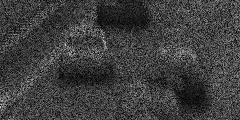
\includegraphics[width=\linewidth]{cars/coded snapshot, T = 7.png}
		\caption{$T=7$}
	\end{subfigure}\\
	\begin{subfigure}{0.2\linewidth}
		\centering
		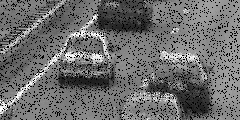
\includegraphics[width=\linewidth]{cars/coded snapshot weighted averaging, T = 3.png}
		\caption{$T=3$}
	\end{subfigure}
	\begin{subfigure}{0.2\linewidth}
		\centering
		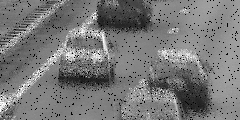
\includegraphics[width=\linewidth]{cars/coded snapshot weighted averaging, T = 5.png}
		\caption{$T=5$}
	\end{subfigure}
	\begin{subfigure}{0.2\linewidth}
		\centering
		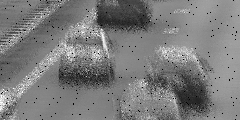
\includegraphics[width=\linewidth]{cars/coded snapshot weighted averaging, T = 7.png}
		\caption{$T=7$}
	\end{subfigure}
	\caption{\\Row 1: Coded Snapshot, displays average value of each pixel\\Row 2: Coded Snapshot, displays weighted average value of each pixel using the code as the weight}
	\label{fig:ccs}
\end{figure}
\begin{figure}[H]
	% \centering
	\begin{subfigure}{0.13\linewidth}
		\centering
		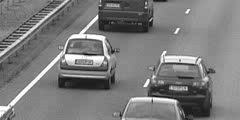
\includegraphics[width=\linewidth]{cars/frame = 1.png}
		\caption{Frame 1}
	\end{subfigure}
	\begin{subfigure}{0.13\linewidth}
		\centering
		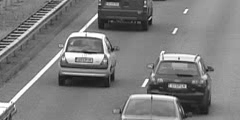
\includegraphics[width=\linewidth]{cars/frame = 2.png}
		\caption{Frame 2}
	\end{subfigure}
	\begin{subfigure}{0.13\linewidth}
		\centering
		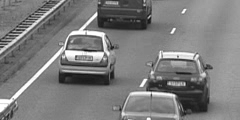
\includegraphics[width=\linewidth]{cars/frame = 3.png}
		\caption{Frame 3}
	\end{subfigure}
	\begin{subfigure}{0.13\linewidth}
		\centering
		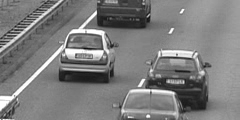
\includegraphics[width=\linewidth]{cars/frame = 4.png}
		\caption{Frame 4}
	\end{subfigure}
	\begin{subfigure}{0.13\linewidth}
		\centering
		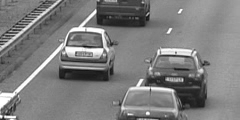
\includegraphics[width=\linewidth]{cars/frame = 5.png}
		\caption{Frame 5}
	\end{subfigure}
	\begin{subfigure}{0.13\linewidth}
		\centering
		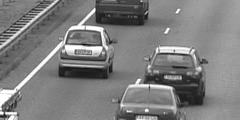
\includegraphics[width=\linewidth]{cars/frame = 6.png}
		\caption{Frame 6}
	\end{subfigure}
	\begin{subfigure}{0.13\linewidth}
		\centering
		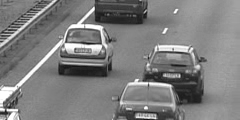
\includegraphics[width=\linewidth]{cars/frame = 7.png}
		\caption{Frame 7}
	\end{subfigure}\\
	\begin{subfigure}{0.13\linewidth}
		\centering
		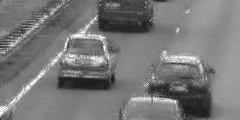
\includegraphics[width=\linewidth]{cars/reconstructed, T = 3, frame = 1.png}
		\caption{Frame = 1}
	\end{subfigure}
	\begin{subfigure}{0.13\linewidth}
		\centering
		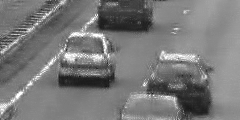
\includegraphics[width=\linewidth]{cars/reconstructed, T = 3, frame = 2.png}
		\caption{Frame = 2}
	\end{subfigure}
	\begin{subfigure}{0.13\linewidth}
		\centering
		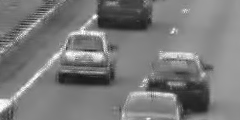
\includegraphics[width=\linewidth]{cars/reconstructed, T = 3, frame = 3.png}
		\caption{Frame = 3}
	\end{subfigure}\\
	\begin{subfigure}{0.13\linewidth}
		\centering
		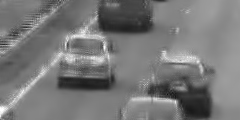
\includegraphics[width=\linewidth]{cars/reconstructed, T = 5, frame = 1.png}
		\caption{Frame = 1}
	\end{subfigure}
	\begin{subfigure}{0.13\linewidth}
		\centering
		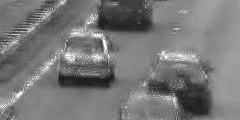
\includegraphics[width=\linewidth]{cars/reconstructed, T = 5, frame = 2.png}
		\caption{Frame = 2}
	\end{subfigure}
	\begin{subfigure}{0.13\linewidth}
		\centering
		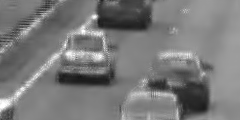
\includegraphics[width=\linewidth]{cars/reconstructed, T = 5, frame = 3.png}
		\caption{Frame = 3}
	\end{subfigure}
	\begin{subfigure}{0.13\linewidth}
		\centering
		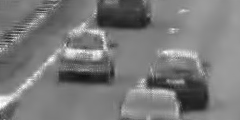
\includegraphics[width=\linewidth]{cars/reconstructed, T = 5, frame = 4.png}
		\caption{Frame = 4}
	\end{subfigure}
	\begin{subfigure}{0.13\linewidth}
		\centering
		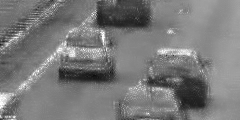
\includegraphics[width=\linewidth]{cars/reconstructed, T = 5, frame = 5.png}
		\caption{Frame = 5}
	\end{subfigure}\\
	\begin{subfigure}{0.13\linewidth}
		\centering
		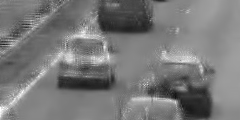
\includegraphics[width=\linewidth]{cars/reconstructed, T = 7, frame = 1.png}
		\caption{Frame = 1}
	\end{subfigure}
	\begin{subfigure}{0.13\linewidth}
		\centering
		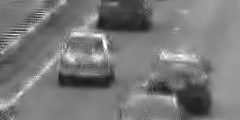
\includegraphics[width=\linewidth]{cars/reconstructed, T = 7, frame = 2.png}
		\caption{Frame = 2}
	\end{subfigure}
	\begin{subfigure}{0.13\linewidth}
		\centering
		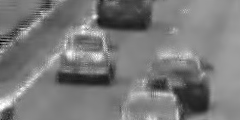
\includegraphics[width=\linewidth]{cars/reconstructed, T = 7, frame = 3.png}
		\caption{Frame = 3}
	\end{subfigure}
	\begin{subfigure}{0.13\linewidth}
		\centering
		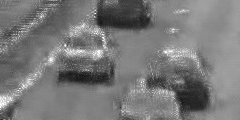
\includegraphics[width=\linewidth]{cars/reconstructed, T = 7, frame = 4.png}
		\caption{Frame = 4}
	\end{subfigure}
	\begin{subfigure}{0.13\linewidth}
		\centering
		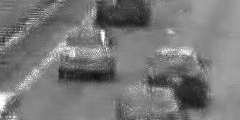
\includegraphics[width=\linewidth]{cars/reconstructed, T = 7, frame = 5.png}
		\caption{Frame = 5}
	\end{subfigure}
	\begin{subfigure}{0.13\linewidth}
		\centering
		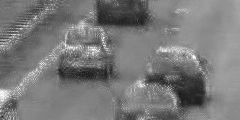
\includegraphics[width=\linewidth]{cars/reconstructed, T = 7, frame = 6.png}
		\caption{Frame = 6}
	\end{subfigure}
	\begin{subfigure}{0.13\linewidth}
		\centering
		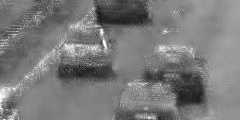
\includegraphics[width=\linewidth]{cars/reconstructed, T = 7, frame = 7.png}
		\caption{Frame = 7}
	\end{subfigure}
	\caption{\\Row 1: Original Images\\Row 2: Reconstructed Images for $T=3$, RMSE = 0.12107\\Row 3: Reconstructed Images for $T=5$, RMSE = 0.14484\\Row 4: Reconstructed Images for $T=7$, RMSE = 0.16047}
	\label{fig:cf}
\end{figure}
\begin{figure}[H]
	\centering
	\begin{subfigure}{0.2\linewidth}
		\centering
		
\includegraphics[width=\linewidth]{flame/coded snapshot, T = 3.png}
		\caption{$T=3$}
	\end{subfigure}
	\begin{subfigure}{0.2\linewidth}
		\centering
		
\includegraphics[width=\linewidth]{flame/coded snapshot, T = 5.png}
		\caption{$T=5$}
	\end{subfigure}
	\begin{subfigure}{0.2\linewidth}
		\centering
		
\includegraphics[width=\linewidth]{flame/coded snapshot, T = 7.png}
		\caption{$T=7$}
	\end{subfigure}\\
	\begin{subfigure}{0.2\linewidth}
		\centering
		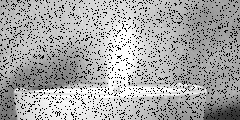
\includegraphics[width=\linewidth]{flame/coded snapshot weighted averaging, T = 3.png}
		\caption{$T=3$}
	\end{subfigure}
	\begin{subfigure}{0.2\linewidth}
		\centering
		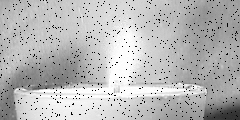
\includegraphics[width=\linewidth]{flame/coded snapshot weighted averaging, T = 5.png}
		\caption{$T=5$}
	\end{subfigure}
	\begin{subfigure}{0.2\linewidth}
		\centering
		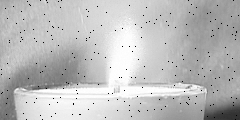
\includegraphics[width=\linewidth]{flame/coded snapshot weighted averaging, T = 7.png}
		\caption{$T=7$}
	\end{subfigure}
	\caption{\\Row 1: Coded Snapshot, displays average value of each pixel\\Row 2: Coded Snapshot, displays weighted average value of each pixel using the code as the weight}
	\label{fig:fcs}
\end{figure}
\begin{figure}[H]
	% \centering
	\begin{subfigure}{0.13\linewidth}
		\centering
		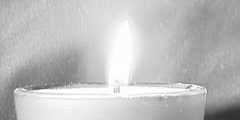
\includegraphics[width=\linewidth]{flame/frame = 1.png}
		\caption{Frame 1}
	\end{subfigure}
	\begin{subfigure}{0.13\linewidth}
		\centering
		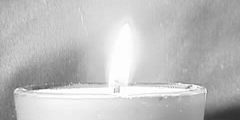
\includegraphics[width=\linewidth]{flame/frame = 2.png}
		\caption{Frame 2}
	\end{subfigure}
	\begin{subfigure}{0.13\linewidth}
		\centering
		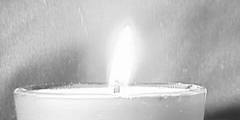
\includegraphics[width=\linewidth]{flame/frame = 3.png}
		\caption{Frame 3}
	\end{subfigure}
	\begin{subfigure}{0.13\linewidth}
		\centering
		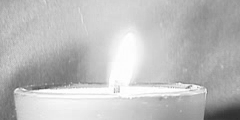
\includegraphics[width=\linewidth]{flame/frame = 4.png}
		\caption{Frame 4}
	\end{subfigure}
	\begin{subfigure}{0.13\linewidth}
		\centering
		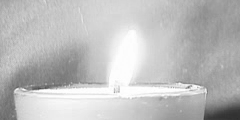
\includegraphics[width=\linewidth]{flame/frame = 5.png}
		\caption{Frame 5}
	\end{subfigure}
	\begin{subfigure}{0.13\linewidth}
		\centering
		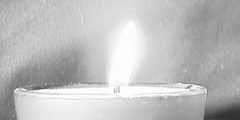
\includegraphics[width=\linewidth]{flame/frame = 6.png}
		\caption{Frame 6}
	\end{subfigure}
	\begin{subfigure}{0.13\linewidth}
		\centering
		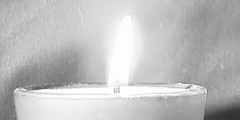
\includegraphics[width=\linewidth]{flame/frame = 7.png}
		\caption{Frame 7}
	\end{subfigure}\\
	\begin{subfigure}{0.13\linewidth}
		\centering
		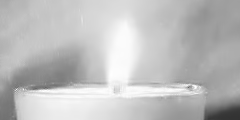
\includegraphics[width=\linewidth]{flame/reconstructed, T = 3, frame = 1.png}
		\caption{Frame = 1}
	\end{subfigure}
	\begin{subfigure}{0.13\linewidth}
		\centering
		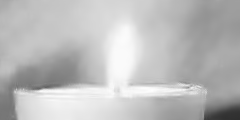
\includegraphics[width=\linewidth]{flame/reconstructed, T = 3, frame = 2.png}
		\caption{Frame = 2}
	\end{subfigure}
	\begin{subfigure}{0.13\linewidth}
		\centering
		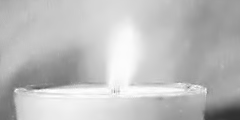
\includegraphics[width=\linewidth]{flame/reconstructed, T = 3, frame = 3.png}
		\caption{Frame = 3}
	\end{subfigure}\\
	\begin{subfigure}{0.13\linewidth}
		\centering
		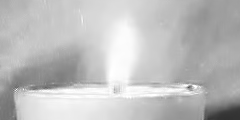
\includegraphics[width=\linewidth]{flame/reconstructed, T = 5, frame = 1.png}
		\caption{Frame = 1}
	\end{subfigure}
	\begin{subfigure}{0.13\linewidth}
		\centering
		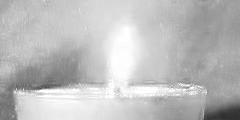
\includegraphics[width=\linewidth]{flame/reconstructed, T = 5, frame = 2.png}
		\caption{Frame = 2}
	\end{subfigure}
	\begin{subfigure}{0.13\linewidth}
		\centering
		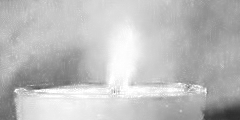
\includegraphics[width=\linewidth]{flame/reconstructed, T = 5, frame = 3.png}
		\caption{Frame = 3}
	\end{subfigure}
	\begin{subfigure}{0.13\linewidth}
		\centering
		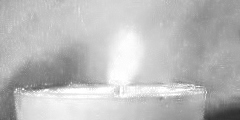
\includegraphics[width=\linewidth]{flame/reconstructed, T = 5, frame = 4.png}
		\caption{Frame = 4}
	\end{subfigure}
	\begin{subfigure}{0.13\linewidth}
		\centering
		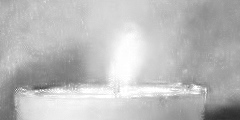
\includegraphics[width=\linewidth]{flame/reconstructed, T = 5, frame = 5.png}
		\caption{Frame = 5}
	\end{subfigure}\\
	\begin{subfigure}{0.13\linewidth}
		\centering
		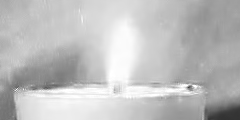
\includegraphics[width=\linewidth]{flame/reconstructed, T = 7, frame = 1.png}
		\caption{Frame = 1}
	\end{subfigure}
	\begin{subfigure}{0.13\linewidth}
		\centering
		\includegraphics[width=\linewidth]{flame/reconstructed, T = 7, frame = 2.png}
		\caption{Frame = 2}
	\end{subfigure}
	\begin{subfigure}{0.13\linewidth}
		\centering
		\includegraphics[width=\linewidth]{flame/reconstructed, T = 7, frame = 3.png}
		\caption{Frame = 3}
	\end{subfigure}
	\begin{subfigure}{0.13\linewidth}
		\centering
		\includegraphics[width=\linewidth]{flame/reconstructed, T = 7, frame = 4.png}
		\caption{Frame = 4}
	\end{subfigure}
	\begin{subfigure}{0.13\linewidth}
		\centering
		\includegraphics[width=\linewidth]{flame/reconstructed, T = 7, frame = 5.png}
		\caption{Frame = 5}
	\end{subfigure}
	\begin{subfigure}{0.13\linewidth}
		\centering
		\includegraphics[width=\linewidth]{flame/reconstructed, T = 7, frame = 6.png}
		\caption{Frame = 6}
	\end{subfigure}
	\begin{subfigure}{0.13\linewidth}
		\centering
		\includegraphics[width=\linewidth]{flame/reconstructed, T = 7, frame = 7.png}
		\caption{Frame = 7}
	\end{subfigure}
	\caption{\\Row 1: Original Images\\Row 2: Reconstructed Images for $T=3$, RMSE = 0.025309\\Row 3: Reconstructed Images for $T=5$, RMSE = 0.028312\\Row 4: Reconstructed Images for $T=7$, RMSE = 0.032038}
	\label{fig:ff}
\end{figure}
\end{document}